\documentclass[11pt,a4paper,margin=0.5in]{report}

\usepackage[utf8]{inputenc}
\usepackage[francais]{babel}
\usepackage[margin=1in,footskip=0.25in]{geometry}
\usepackage{graphicx}
\usepackage[document]{ragged2e}
\usepackage{hyperref}

\title{ 
\includegraphics[scale=0.33]{m3.png} \\[0.25in]Modular Mind Mapping - M3 \\ UPMC M2 STL TPDEV Projet}
\author{Elias Boutaleb}
\date{\today}

\begin{document}

\maketitle
\tableofcontents

\chapter{Introduction}

\begin{center}
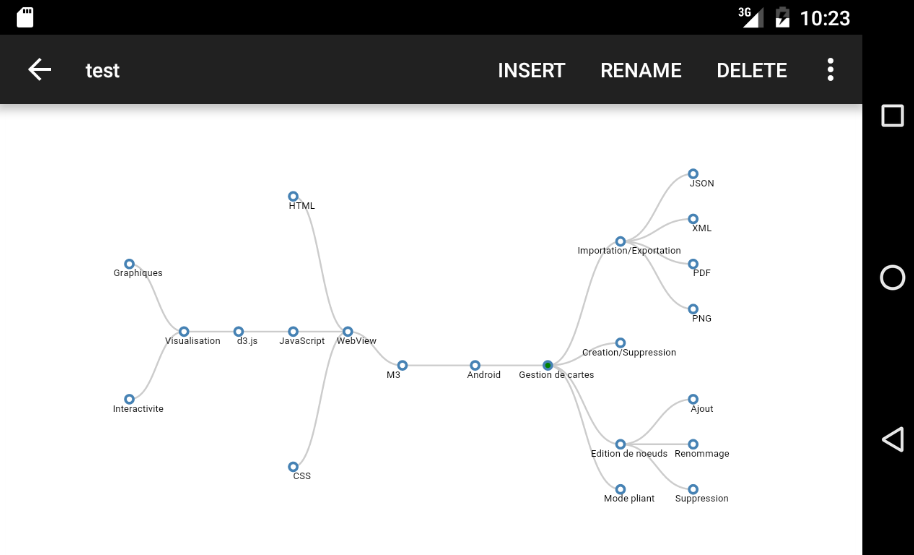
\includegraphics[scale=0.5]{mm.png} \\[0.25in]
\end{center}

\section{Contexte}

Modular Mind Mapping (M3) est un logiciel de cartographie conceptuelle (mindmapping) qui permet d'organiser des informations de manière
visuelle sous forme d'arborescence. \\[0.25in]

Le concept de mindmapping est simple: il s'agit de cr
On part d'un thème donné, puis on y associe différentes idées, des images, d'autres mots, des hyperliens.

\begin{figure}[!ht]
  \centering
    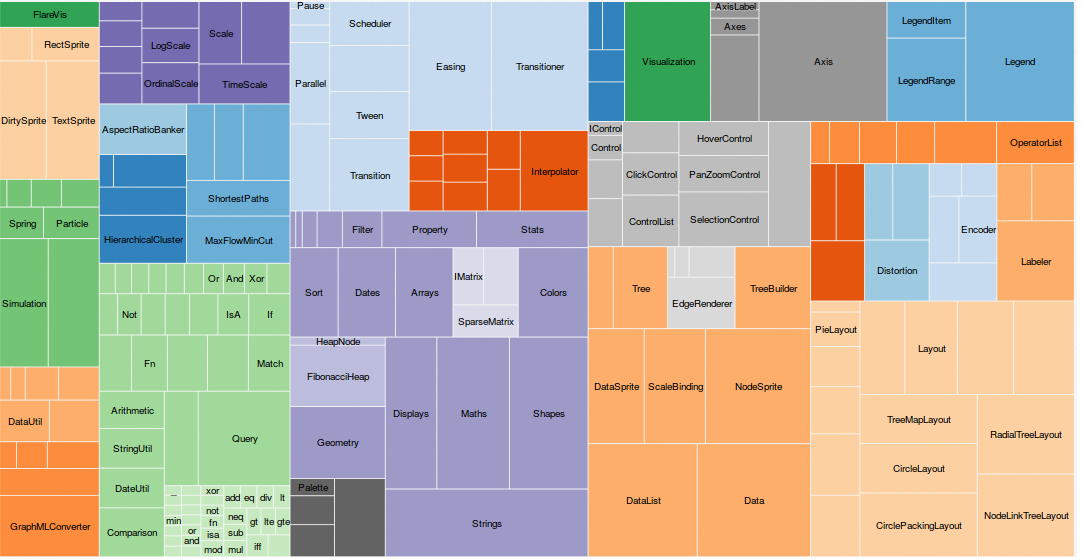
\includegraphics[width=1\textwidth]{d31.png} \\[0.25in]
  \centering
    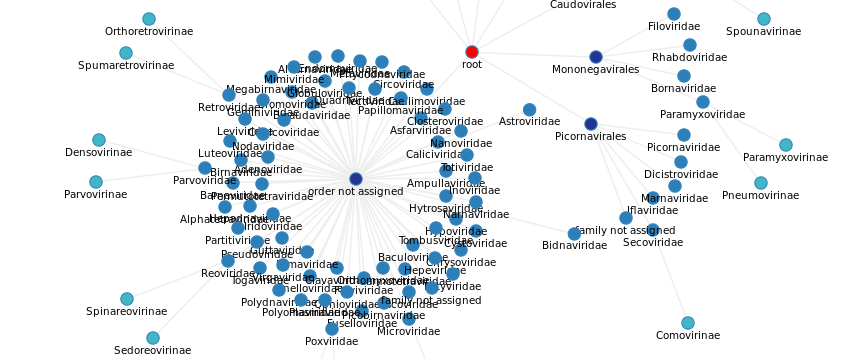
\includegraphics[width=1\textwidth]{d33.png} \\[0.25in]
  \caption{M3 utilise le framework de visualisation de données d3.js, qui permet de représenter un ensemble de données de manière visuelle et dynamique.}
\end{figure}

\clearpage

Il existe déjà plusieurs applications de ce type sur le Google Play Store mais plusieures choses ne convenaient
pas au développeur de M3:

\begin{itemize}
\item{la plupart de ces applications sont gratuites, mais des fonctionnalités interessantes comme l'insertion
de médias (images, sons) se trouvent dans une version payante.}

\begin{figure}[!ht]
  \caption{iMindMap, dont la version complète coûte 20 euros par an}
  \centering
    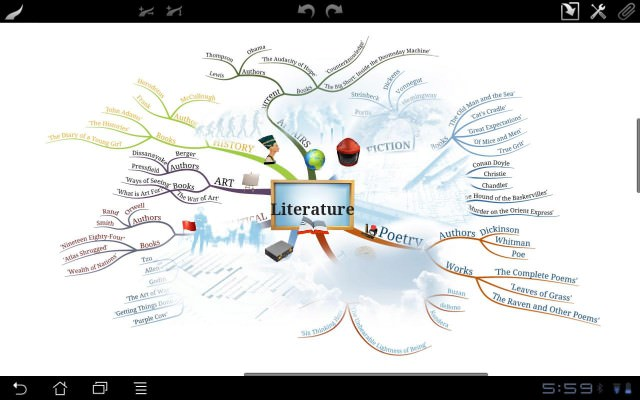
\includegraphics[width=1\textwidth]{ex1.jpg}
\end{figure}

\item{soit elles sont limitées dans leurs options d'importation et exportation des cartes.}

\begin{figure}[!ht]
  \caption{SimpleMind}
  \centering
    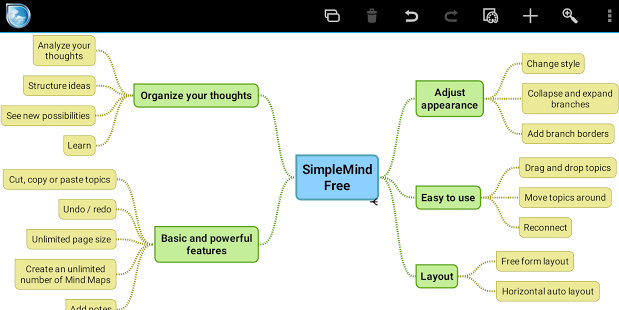
\includegraphics[width=1\textwidth]{unnamed.png}
\end{figure}

\end{itemize}

\clearpage

Le créateur de M3 a donc estimé qu'il pourrait être intéressant de pouvoir intégrer les capacités de visualisation de données de d3.js\footnote{\url{http://d3js.org/}} à une mindmap, ce qui n'a pas encore été fait jusqu'à présent.
M3 se passera des limitations associées à ce type d'application:

\begin{itemize}
\item pas de version payante, l'unique version (gratuite) contient toutes les fonctionnalités offertes
\item le code source est disponible librement. Tout utilisateur (programmeur ou non) peut contribuer à son amélioration.
\end{itemize}

\section{Fonctionnalités}

Pour l'instant, M3 dispose des fonctionnalités suivantes :

\begin{itemize}
\item Les cartes peuvent être chargées ou enregistrées sur l'appareil au format JSON.
\item Création et suppression de cartes.
\item Edition des noeuds (ajout, suppression, renommage, changement de l'agencement.
\item Mode de visualisation d'arbre pliable disponible.
\end{itemize}

\chapter{Description de l'interface}


\begin{figure}[!ht]
  \centering
    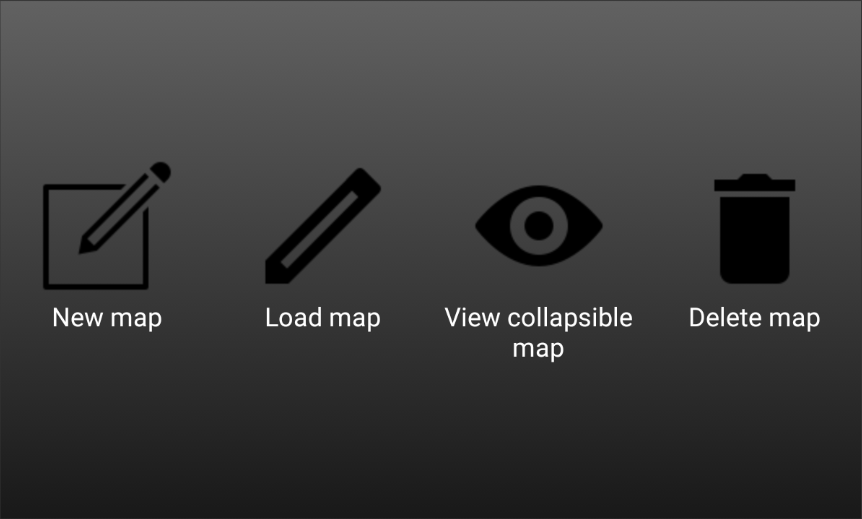
\includegraphics[width=1\textwidth]{dashb.png} \\[0.25in]
  \caption{DashBoard de M3. Il est possible de créer une nouvelle carte, d'en charger une déja existante, ou bien d'en supprimer.}
\end{figure}

\begin{figure}[!ht]
  \centering
    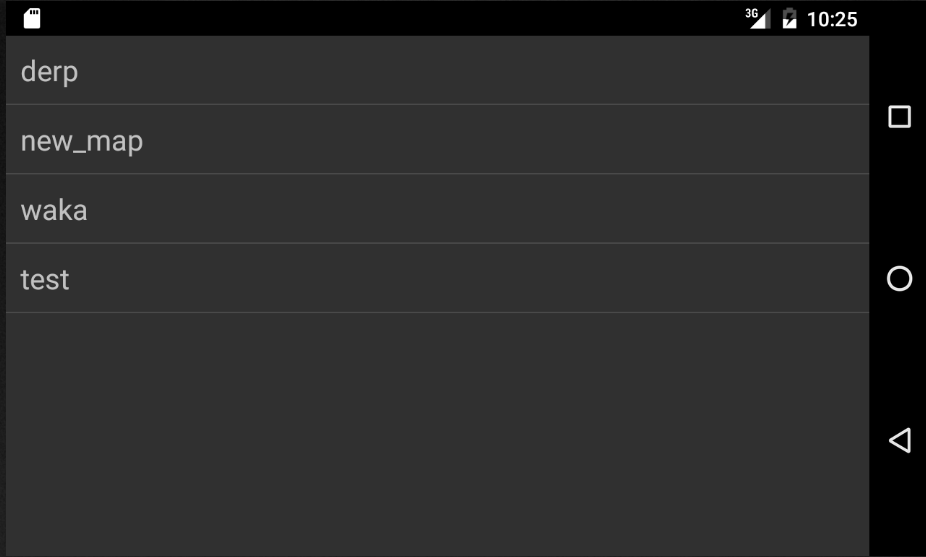
\includegraphics[width=1\textwidth]{choice.png} \\[0.25in]
    \caption{La liste des fichiers stockés dans la mémoire de l'appareil.}
Cette liste est affichée pour sélectionner une carte à manipuler.
\end{figure}


\begin{figure}[!ht]
  \centering
    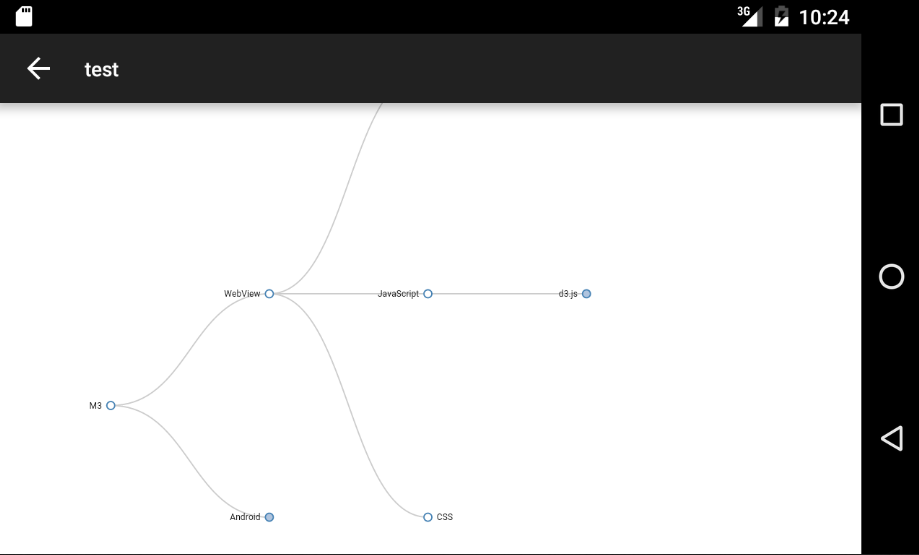
\includegraphics[width=1\textwidth]{coll.png} \\[0.25in]
    \caption{Les cartes peuvent aussi être vues sous la forme d'un arbre pliant.}
\end{figure}


\clearpage

\chapter{Extensions et améliorations}

\section{Contraintes}
\begin{itemize}
\item Il y a des problèmes intermittents de performance dûs à l'utilisation d'un navigateur.
\item L'interface utlisateur est bancale: la manipulation des noeuds se fait uniquement par l'intermédiaire de 
boutons qui communiquent avec le code JavaScript de l'application.
\item En conséquence, l'arrangement des noeuds dans les cartes est rigide et ne peut être modifié librement.
\end{itemize}

\section{Extensions et améliorations}

\begin{itemize}
\item Exportation de cartes aux formats PNG et PDF
\item Importation de cartes FreeMind XML (.mm).
\item Import de données qui seront visualisées
\item Intégrer la visualisation de graphs d3 aux cartes
\item L'insertion d'images est envisagée.
\item Changement du fond, des couleurs
\item Utilisation de structures propres à Android (TextView/ImageView) pour une manipulation interactive de la carte plus dynamique
\end{itemize}

\end{document}
